\documentclass[10pt,english]{article}

\usepackage{amsfonts,url,tikz}
\usepackage{amsmath}
\usepackage{amssymb}
\usepackage{hyperref}

% Paper setup
\evensidemargin=0in
\oddsidemargin=0in
\textwidth=6.25in
\topmargin=-0.5in
\headheight=0.0in
\headsep=0.5in
\textheight=9.0in
\footskip=0.5in

%\usepackage{fixltx2e}

\newcommand{\Interior}[1]{\ensuremath{{#1}^{\circ}}}
\newcommand{\Closure}[1]{\ensuremath{\overline{#1}}}
\newcommand{\Complement}[1]{\ensuremath{{#1}^{c}}}

\newcommand{\Expect}{\ensuremath{\mathrm{E}}}
\newcommand{\vecnot}{\underline}
\newcommand{\RealNumbers}{\mathbb{R}}
\newcommand{\RationalNumbers}{\mathbb{Q}}
\newcommand{\ComplexNumbers}{\mathbb{C}}
\newcommand{\Real}{\mathrm{Re}}
\newcommand{\Span}{\mathrm{span}}
\newcommand{\Rank}{\mathrm{rank}}
\newcommand{\Nullity}{\mathrm{nullity}}
\newcommand{\Trace}{\mathrm{tr}}
\newcommand{\Diag}{\mathrm{diag}}
\DeclareMathOperator*{\esssup}{ess\,sup}
\newcommand{\dd}{\mathrm{d}}



\begin{document}

\title{ECE 586: Vector Space Methods \\ Lecture 6: Frequently Asked Questions}
\author{Henry D. Pfister \\ Duke University}
\date{September 14, 2020}

\maketitle

Here we give a list of questions, and their answers, that were submitted by students after watching the flip video.

\section{Continuity}

\paragraph{On the Continuity slide, you introduce a function $f$ between two metric spaces. Are the metric spaces themselves a part of the domain and codomain of $f$ or are $X$ and $Y$ exclusively the domain and the codomain? I am primarily confused as to the difference between a metric space and a set.} 

Functions are defined between sets.
So, the domain and codomain are the sets $X$ and $Y$.
A metric space is a set that has a well-defined ``distance'' between any two elements of the set (section 2.1 in notes).
The definition of continuity only applies to a function $f\colon X \to Y$ between two metric spaces because one cannot define continuity without metrics on $X$ and $Y$.


\paragraph{Could you elaborate on the definition of uniformly continuous? I did not understand how $\delta$ can be ``chosen independently of $x$" or what this means.}

For $f:X \to Y$, the definition of continuity is: For all $x\in X$ and all $\epsilon > 0$, there is a $\delta >0$ such that, for all $z \in B_X (x,\delta)$, we have $d_Y (f(x),f(z)) < \epsilon$.
Since the $\exists\delta$ occurs after the $\forall x$, the choice of $\delta$ is allowed to depend on $x$.

In contrast, the definition of uniform continuity is: For all $\epsilon > 0$, there is a $\delta >0$ such that, for all $x\in X$ and all $z \in B_X (x,\delta)$, we have $d_Y (f(x),f(z)) < \epsilon$.
Since the $\forall x$ occurs after $\exists\delta$, the choice of $\delta$ is not allowed to depend on $x$.

As an example, for $X=(0,\infty)\subset \mathbb{R}$ with absolute distance, the function $f(x)=x^2$ is not uniformly continuous.
Intuitively, this is because its slope grows without bound as $x$ increases.
To see this formally, let $\epsilon = 1$ and, for any $\delta >0$, choose $x=1/\delta$.
Then, $z=x+\delta/2$ satisfies $|x^2 - z^2| = 1+\delta^2 / 4 > \epsilon$.
Thus, $f$ is not uniformly continuous.


\paragraph{How to use Lipschitz continuity in application? Why we define this kind of continuity?} % Similar question \paragraph{Why mention Lipschitz continuous? Are there any applications that Lipschitz continuous is more useful than the ordinary continuous condition?}

Lipschitz continuity is a strong form of continuity that is very useful in practice.
For example, it is easy to verify that, if $f\colon X \to Y$ is Lipschitz-$L_f$ and $g \colon Y \to Z$ is Lipschitz-$L_g$, then $g \circ f \colon X \to Z$ is Lipschitz-$L_f L_g$

As an application, recall that a contraction is Lipschitz-$\gamma$ for some $\gamma <1$.
Thus, composing a contraction $f \colon X \to X$ with itself $n$ times gives a function that is Lipschitz-$\gamma^n$.
In other words, contraction mapping theorem basically says that composing a contraction with itself eventually gives a Lipschitz-0 function whose output value is independent of the input value.

 
\paragraph{Could a function be Lipschitz continuous if it is not one-to-one?}

Lipschitz continuous does not relate to whether a function is one-on-one. The following figure shows four functions, which are (1, red) Lipschitz continuous and one-on-one; (2, black) Lipschitz continuous but not one-on-one; (3, blue) not Lipschitz continuous but one-on-one; (4, green) neither Lipschitz continuous nor one-on-one.

%\begin{figure*}[h]
\begin{center}
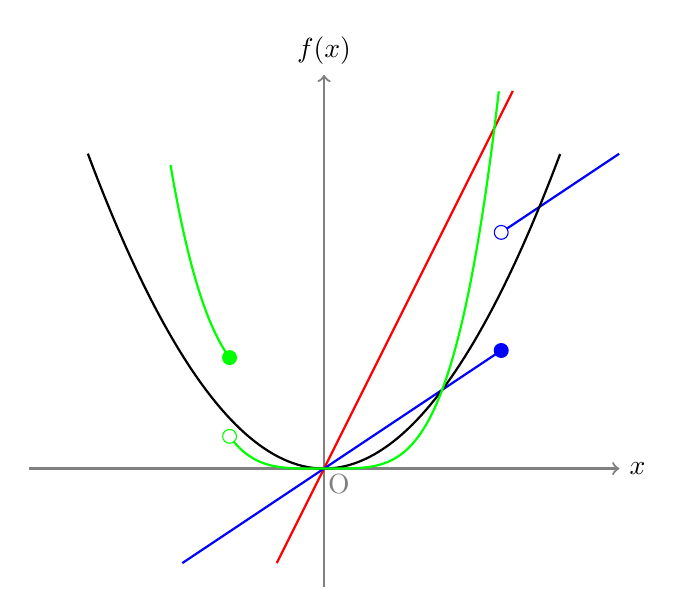
\begin{tikzpicture}[xscale=1.5]
  \draw [thick, draw=gray, ->] (-2.5,0) -- (2.5,0) node[right, black] {$x$};
  \draw [thick, draw=gray, ->] (0,-1.5) -- (0,5) node[above, black] {$f(x)$};
  \draw [red, thick, domain=-0.4:1.6, samples=100] plot(\x, {((3*\x)});
  \draw [blue, thick, domain=-1.2:1.5, samples=100] plot(\x, {((\x)});
  \draw [blue, thick, domain=1.5:2.5, samples=100] plot(\x, {((\x)+1.5});
  \node[circle,draw=blue, fill=blue, inner sep=0pt,minimum size=5pt] at (1.5,1.5) {};
  \node[circle,draw=blue, fill=white, inner sep=0pt,minimum size=5pt] at (1.5,3) {};
  \draw [black, thick, domain=-2:2, samples=100] plot(\x, {(\x*\x)});
  \draw [green, thick, domain=-1.3:-0.8, samples=100] plot(\x, {(\x*\x*\x*\x+1)});
  \draw [green, thick, domain=-0.8:1.48, samples=100] plot(\x, {(\x*\x*\x*\x)});
  \node[circle,draw=green, fill=green, inner sep=0pt,minimum size=5pt] at (-0.8,1.4096) {};
  \node[circle,draw=green, fill=white, inner sep=0pt,minimum size=5pt] at (-0.8,0.4096) {};
  \draw (0.3,-0.2) node[left, text=gray]{O};
\end{tikzpicture}
\end{center}
%\end{figure*}

\paragraph{Does Lipschitz continuity on $A$ essentially require that the derivative not approach infinity on $A$?}

Yes.
For $A=[a,b]$ and a differentiable function $f\colon X \to \mathbb{R}$, the Lipschitz constant satisfies (by definition)
\[ L \geq \frac{|f(y) - f(x)|}{|y-x|} \]
for all $x,y \in A$.
Letting $y=x+\delta$ and taking the limit as $\delta \to 0$ also shows that $L \geq f'(x)$ for all $x \in A$.

 


\paragraph{How is Lipschitz continuity different from the plain definition of continuity?}

One can show that the function $f\colon [0,\infty) \to [0,\infty)$ defined by $f(x) = \sqrt{x}$ is uniformly continuous but not Lipschitz continuous because $f'(0^+)=\infty$. 


\iffalse

\paragraph{Dawei Xi: Why do we define three different continuous functions, continuous function, uniformly continuous, Lipschitz continuous?}



\paragraph{Why is for standard metric space (e.g. used in real analysis), $X = \mathbb{R}$, and for Euclidean space $X = \mathbb{R}^n$?}




\fi

\section{Properties of Real Numbers}

\paragraph{I am not very clear with the difference between the supremum and the maximum and the infimum and the minimum. Could you give some examples where they are equal and some where they are not?}
The supremum is simply the smallest value that upper bounds all values in a set $X$. Sometimes (e.g. when the set $X$ is compact),this coincides with the maximum. An example where maximum and supremum are \textit{not} the same is the interval [0,1), where 1 is the supremum, but the maximum is undefined.

\paragraph{What is the intuition behind infimum and supremum?}

This might be a good picture to keep in mind (\href{https://en.wikipedia.org/wiki/Infimum_and_supremum#/media/File:Illustration_of_supremum.svg}{\textbf{Click here for image link}}). A set $M\subset \mathbb{R}$ can have many upper bounds, but one of these upper bounds is the smallest, and that is precisely $\text{sup}(M)$.


\paragraph{If we have a sequence of logistic functions (of the general form $f_n(x) = \frac{1}{1+e^{-nx}}$), each considered continuous, that converge to a step function, can the step function still be called continuous?}
Indeed, this sequence converges to the step function, but the step function itself is not continuous.
Let's take the contrapositive of the last theorem on sequences of continuous functions.
\begin{itemize}
\item This yields:
``$f$ is not continuous $\Rightarrow$ not all $f_n$ are continuous OR $f_n$ does not converge uniformly to $f$''.
\item Since in your example we \textit{know} the $f_n$'s \textit{are} continuous, this means they must not \textit{uniformly} converge to $f$.
\end{itemize}
The take-away here is that, for the limit function $f$ to be continuous, you need 2 ingredients: $f_n$ must be continuous for all $n$, and $f_n$ must converge \textit{uniformly} to $f$.


\paragraph{Is the supremum used mainly for open sets whereas the maximum can be more easily applied on a closed set?}
If you think beyond just the real line $\mathbb{R}$, there are plenty of cases where we might see a supremum over an open set $A$.
e.g. consider the function $f(x,y) = -(x^2 + y^2)$ over the set $A = \{(x,y) | x^2 + y^2 < 5\}$. Here, you can check that $A$ is an open set, but the supremum of $f(A)$ (and coincidentally, the maximum of $f(A)$) is $0$ and occurs at $x=y=0$.

Conversely, the set $\mathbb{R}$ is itself closed, and its supremum is $+\infty$, yet its maximum is undefined.
Later, we will see that, if a set $A\in\mathbb{R}$ is compact, then its supremum and maximum are the same.
This follows from continuous functions (such as $f(x)=x$) achieving their supremum as a maximum.


\paragraph{What's the difference between uniform and pointwise convergence?}
Pointwise convergence means that, for all $x$, $f_n(x)$ converges to $f(x)$ -- this means that, for every $x$ and $\epsilon>0$, we can find an $N = N(x,\epsilon)$ beyond which $d(f_n(x),f(x))<\epsilon$.
Uniform convergence means that, for all $\epsilon>0$, we can find an $N = N(\epsilon)$ beyond which $d(f_n(x),f(x))<\epsilon$, for all $x$. Note that $N$ here does not depend on $x$, only $\epsilon$ -- intuitively, this suggests that the convergence rate of $f_n(x)$ to $f(x)$ cannot become arbitrarily slow for some $x\in X$. 

This is not the case for pointwise convergence (where $N$ might depend on both $x$ and $\epsilon$).
Note that uniform convergence \textit{implies} pointwise convergence, but not vice versa.




\paragraph{How does one properly define the "extended" real numbers? I thought that there was in issue in treating negative infinity and infinity as if they were numbers (i.e. the definition has a union of the reals with plus / minus infinity).}

This is a good question that exposes the fuzziness surrounding terms like ``the real numbers".
The \textit{metric space} of extended real numbers can be defined by choosing $\overline{\mathbb{R}} \triangleq \mathbb{R} \cup \{ \infty,-\infty\}$ and defining a distance that satisfies the properties of a metric such as
\[ d_{\overline{\mathbb{R}}} (x,y) \triangleq \left|\frac{x}{1+|x|} - \frac{y}{1+|y|} \right|, \]
where $\frac{x}{1+|x|}\big|_{x=\pm\infty} \triangleq \pm 1$.

In general, the extended real numbers cannot be assigned a more complicated mathematical structure (e.g., think group, ring, field, or vector space) because there is no reasonable way to define $\infty + (- \infty)$.

\paragraph{Why is the set of extended real numbers bigger than the set of real numbers? Isn't the set $\{-\infty, \infty\}$ a subset of the real numbers?}

No, the symbols $\infty,-\infty$ are not real numbers.



\end{document}
